\documentclass[a4paper,12pt]{article}
\usepackage[utf8]{inputenc}
\usepackage{longtable}
\usepackage{geometry}
\usepackage{hyperref}
\usepackage{array}
\usepackage{caption}
\usepackage{booktabs}
\geometry{margin=1in}
\usepackage{graphicx}
\usepackage{float}

\title{Software Requirements Specification\\Taxi Tap by Git It Done}
\date{}

\begin{document}

\maketitle

\begin{figure}[H]
  \centering
  
\includegraphics[width=0.5\textwidth]{LogoGroup.png} 
\end{figure}

\begin{figure}[H]
  \centering
  
\includegraphics[width=0.5\textwidth]{LogoTaxiTap.png} 
\end{figure}

\newpage

\tableofcontents
\newpage

\section{Introduction}
Taxi Tap is a mobile platform designed to revolutionize South Africa’s minibus taxi industry by digitizing route information, eliminating the need for constant hooting, and creating a semi-structured booking system while preserving the flexibility that makes taxis an essential mode of transport. The system connects passengers and taxi operators through a location-aware mobile application that facilitates taxi requests, communicates passenger locations, manages payments, and provides real-time vehicle tracking – all without fundamentally changing the existing system's multi-passenger, flexible route nature.

\section{User Characteristics}

The users of the Taxi Tap system are expected to fit into the following groups:

\subsection{Driver User Characteristics}

\begin{longtable}{>{\raggedright}p{5cm} p{10cm}}
\toprule
\textbf{Attribute} & \textbf{Description} \\
\midrule
Familiarity with Mobile Technology & Varies widely: Some drivers may be tech-comfortable while others may struggle with apps. \\
Access to Reliable Internet and Data & Often limited or inconsistent, drivers operate in areas with poor signal or data is expensive. \\
Preferred Language and Communication Style & They may prefer local languages (e.g. Zulu, Xhosa, Sesotho). \\
Attention Capacity While Driving & Must be able to use the app while operating a vehicle, requiring minimal taps and distractions. \\
Trust and Skepticism Toward New Technology & May be skeptical of new digital systems due to fear of replacement, surveillance, or fare manipulation. \\
Goals and Incentives for Using the App & Wants more passengers, quicker pickups, and less idle time without changing their daily routine. \\
\bottomrule
\end{longtable}

\subsection{Passenger User Characteristics}

\begin{longtable}{>{\raggedright}p{5cm} p{10cm}}
\toprule
\textbf{Attribute} & \textbf{Description} \\
\midrule
Digital Literacy & Ranges from students and workers (tech-savvy) to commuters with limited app experience. \\
Access to Reliable Internet and Data & Frequently encounters low or no connectivity, especially in transit \\
Reasons for Using the Platform & It seeks reliable transport, less waiting, and a safer way to locate and use taxis. \\
Preferred Language and Communication Style & They may prefer local languages (e.g. Zulu, Xhosa, Sesotho). \\
App Usage Context (Where \& When) & Often uses the app in crowded, noisy, or busy settings like taxi ranks. \\
Concerns Around Trust and Safety & Wants to be sure drivers are legitimate and that their location and personal data are protected. \\
Platform Interaction Needs & Need to discover taxis, request rides, track driver arrival, and receive ride notifications. \\
\bottomrule
\end{longtable}

\section{User Stories}

\subsection{Passenger User Stories}

\begin{longtable}{>{\raggedright}p{4cm} p{6cm} p{5cm}}
\toprule
\textbf{User Story} & \textbf{Acceptance Criteria} & \textbf{Definition of Done} \\
\midrule
Account Registration \& Login & As a passenger, I want to sign up and log in to my account, so that I can securely access and use the Taxi Tap app. & Given that I am on the app’s welcome screen, When I choose “Sign Up” or “Log In” and enter valid details, Then I should be authenticated and taken to the home screen. \\
& & Based on my input criteria, I am taken to the home page of Taxi Tap \\ \midrule
View Available Taxis and Routes & As a passenger, I want to view available taxis and their routes on a map, so that I can choose one that matches my travel needs. & Given I am logged in, When I open the home screen, Then I should see nearby taxis on a map with route or destination labels. \\
& & The map displays icons of nearby taxis, including route or destination tags, when available. \\ \midrule
Set Pickup and Destination & As a passenger, I want to share my location and set a destination, so that drivers can find and pick me up efficiently. & Given that I have granted location access, When I enter or select a pickup and destination point, Then the app should confirm my trip details and show nearby taxis. \\
& & Pickup and destination are confirmed and displayed; nearby taxis are suggested based on the selected route. \\ \midrule
Book a Seat and Get Confirmation & As a passenger, I want to book a seat on a taxi and receive confirmation, so that I’m guaranteed a spot before the taxi arrives. & Given I’ve selected a taxi, When I tap “Book Seat” and confirm, Then I should receive a booking confirmation and a ride status update. \\
& & A booking confirmation message appears with the selected taxi details and current ride status. \\ \midrule
Track Assigned Taxi in Real-Time & As a passenger, I want to track my assigned taxi in real time, so that I know when and where to expect pickup. & Given my booking is confirmed, When I open the tracking screen, Then I should see the taxi’s live location and estimated time of arrival. \\
& & The assigned taxi is visible on the map with a live location marker and updated ETA. \\ \midrule
Receiving Alerts When Taxi is Nearby & As a passenger, I want to receive alerts when the taxi is nearby, so that I can be ready at the pickup location. & Given the assigned taxi is approaching, When it is within 500 meters, Then I should receive a push notification that it’s nearby. \\
& & A push alert is triggered and received once the taxi enters the defined proximity radius. \\ \midrule
See Available Seats & As a passenger, I want to see how many seats are available, so that I can decide whether to book a seat or wait. & Given I view a taxi on the map or booking screen, When I open its details, Then I should see the number of available seats. \\
& & The number of available seats is clearly shown for each listed or selected taxi. \\ \midrule
Rate Completed Trip & As a passenger, I want to rate my trip after completion, so that I can provide feedback to help improve the service. & Given my ride has ended, When I open the app, Then I should be prompted to leave a 1–5 star rating and optional comments. \\
& & The rating form appears automatically after the ride ends, and feedback is successfully submitted to the system. \\ \midrule
Use App Offline or on Low Bandwidth & As a passenger, I want to use the app offline or on low bandwidth, so that I can still interact with core features in areas with poor connectivity. & Given I have limited internet access, When I open the app, Then I should still be able to view saved routes, taxis, and queue a ride request that sends once reconnected. \\
& & The app functions with cached map data and stores ride requests locally, syncing once connectivity is restored. \\ \midrule
Indicate Drop-Off Point Mid-Trip & As a passenger, I should be able to indicate where I want to be dropped off during the trip. & Given that I’m in a running taxi, When I choose a stop or drop-off location mid-trip, Then the driver should receive an update of my chosen point. \\
& & The app allows drop-off selection, sends update to driver, and displays new estimated drop-off. \\ \midrule
View All Available Stops & As a passenger, I should be able to see all the available stops that are there during my trip. & Given I’m on a selected route, When I view route details, Then I should see a list or map of all possible stops. \\
& & A stop list or map view is shown, detailing all available stops along the route. \\ \midrule
See Estimated Time to Destination & As a passenger, I should be able to see how long it will take to reach my destination or drop-off spot. & Given I’ve set a destination, When I view trip details, Then I should see the estimated time remaining. \\
& & ETA is shown dynamically on screen and updates with real-time traffic and route changes. \\
\bottomrule
\end{longtable}


\subsection{Driver User Stories}

\begin{longtable}{>{\raggedright}p{4cm} p{6cm} p{5cm}}
\toprule
\textbf{User Story} & \textbf{Acceptance Criteria} & \textbf{Definition of Done} \\
\midrule
Account Registration \& Login & As a driver, I want to sign up and log in to my account, so that I can securely access and use the Taxi Tap app. & Given that I am on the app’s welcome screen, When I choose “Sign Up” or “Log In” and enter valid details, Then I should be authenticated and taken to the home screen. \\
& & Based on my input criteria, I am taken to the home page of Taxi Tap \\ \midrule
Announce Route \& Destination & As a driver, I want to input the route I will be taking and the destination, so that passengers can see if I’m heading in their direction. & Given that I’m logged in, When I set my starting point and destination, Then the route is visible to nearby passengers. \\
& & The route is stored and displayed to the eligible passenger's interface. \\ \midrule
Go Online/Offline & As a driver, I want to go online or offline as needed, so that I can control when I am available to receive ride requests. & Given that I’m on the driver dashboard, When I tap “Go Online” or “Go Offline”, Then my status is updated accordingly and affects request visibility. \\
& & The driver's online/offline status is reflected, and the passenger can no longer see the taxi on the map. \\ \midrule
Receive Ride Requests & As a driver, I want to receive ride requests from nearby passengers, so that I can choose which pickups to accept. & Given that I am online and have an active route, When a passenger requests a ride, Then I receive a notification with request details. \\
& & Ride requests from matching passengers are delivered in real-time to the driver’s interface. \\ \midrule
Accept or Decline Requests & As a driver, I want to accept or decline a ride request, so that I can manage my route and taxi capacity efficiently. & Given I have received a ride request, When I tap “Accept” or “Decline”, Then the system updates the request status and notifies the passenger. \\
& & Accepted rides appear on the active list; declined requests are logged and cleared. \\ \midrule
View Passenger Pickup Details & As a driver, I want to see the passenger’s pickup point and basic information, so that I know where to stop and who I’m picking up. & Given that I’ve accepted a booking, When I view the trip summary, Then I should see the passenger’s location and name or contact info. \\
& & Pickup details are accurately displayed on the driver's map and trip screen. \\ \midrule
View Map \& Navigation & As a driver, I want to see a map with passenger pickup and route directions, so that I can navigate efficiently. & Given that I have one or more assigned pickups, When I open the map view, Then I should see my location and passenger's location. \\
& & Live maps with GPS and routing is functional and accurate within the app. \\ \midrule
Update Seat Availability & As a driver, I want to update how many seats are available in my taxi, so that passengers can decide whether to book or wait. & Given that I’ve started a trip or gone online, When I adjust seat count manually, Then, passengers see the updated availability. \\
& & Seat count updates in real time and is reflected in the passenger’s booking screen. \\ \midrule
Receive Alerts for New Requests or Updates & As a driver, I want to receive real-time notifications, so that I don’t miss ride requests or updates while driving. & Given that I am online, When a new request or important event occurs, Then I receive a push notification with the relevant details. \\
& & Push and in-app alerts trigger correctly and lead to actionable pages. \\ \midrule
Work Offline (Partial Functionality) & As a driver, I want to continue using key features even when I’m offline, so that I can operate in areas with poor connectivity. & Given that I am offline or have poor signal, When I open the app, Then I should be able to see cached routes and queue ride requests. \\
& & The app stores critical data locally and syncs changes once reconnected. \\ \midrule
Indicate Taxi Association & As a driver, I should be able to indicate which taxi association I am a part of. & Given I am registering or editing my profile, When I select or input my association, Then it should be linked to my driver profile. \\
& & Association name is stored and reflected in the driver's profile and backend database. \\ \midrule
Receive Route from Association & As a driver, I should be assigned a route by my taxi association. & Given I belong to a taxi association, When I log in or go online, Then the assigned route from the association should appear. \\
& & System pulls assigned route from the association records and displays it on the app. \\ \midrule
Receive Drop-Off Notification & As a driver, I should be notified when a passenger wants to get dropped off. & Given I am currently driving and have active passengers, When a passenger selects a drop-off point, Then I receive an alert with the details. \\
& & Notification appears in real-time and updates route on the driver’s screen. \\
\bottomrule
\end{longtable}

\section{Service Contracts}

\subsection*{User Service Contract}

\begin{enumerate}
  \item \textbf{createUser}
    \begin{itemize}
      \item \textbf{Request:}
      \begin{verbatim}
{
  name: string, 
  phoneNumber: string, 
  password: string
}
      \end{verbatim}
      \item \textbf{Response:}
      \begin{verbatim}
{
  userID: string, 
  createdAt: timestamp
}
      \end{verbatim}
      \item \textbf{Effect:}
      \begin{itemize}
        \item Saves a new user to the database and returns the generated user ID and creation timestamp.
      \end{itemize}
    \end{itemize}

  \item \textbf{LoginUser}
    \begin{itemize}
      \item \textbf{Request:}
      \begin{verbatim}
{
  phoneNumber: string, 
  password: string
}
      \end{verbatim}
      \item \textbf{Response:}
      \begin{verbatim}
{
  token: string, 
  userId: string
}
      \end{verbatim}
      \item \textbf{Effect:}
      \begin{itemize}
        \item Authenticates the user and provides a session token.
      \end{itemize}
    \end{itemize}
\end{enumerate}

\subsection*{Ride Booking Service Contract}

\begin{enumerate}
  \item \textbf{ViewAvailableTaxis}
    \begin{itemize}
      \item \textbf{Request:}
      \begin{verbatim}
{
  userLocation: { latitude: float, longitude: float }
}
      \end{verbatim}
      \item \textbf{Response:}
      \begin{verbatim}
[{
  taxiId: string,
  driverName: string,
  availableSeats: int,
  route: string,
  location: {latitude: float, longitude: float}
}]
      \end{verbatim}
      \item \textbf{Effect:}
      \begin{itemize}
        \item Returns a list of nearby taxis with route, price and seat information.
      \end{itemize}
    \end{itemize}

  \item \textbf{bookSeat}
    \begin{itemize}
      \item \textbf{Request:}
      \begin{verbatim}
{
  userId: string,
  taxiId: string,
  pickupLocation: {latitude: float, longitude: float },
  destination: string
}
      \end{verbatim}
      \item \textbf{Response:}
      \begin{verbatim}
{
  bookingId: string,
  status: confirmed,
  estimatedArrivalTime: timestamp,
  price: double
}
      \end{verbatim}
      \item \textbf{Effect:}
      \begin{itemize}
        \item Reserves a seat in the taxi and returns confirmation.
      \end{itemize}
    \end{itemize}

  \item \textbf{trackTaxi}
    \begin{itemize}
      \item \textbf{Request:}
      \begin{verbatim}
{
  bookingId: string
}
      \end{verbatim}
      \item \textbf{Response:}
      \begin{verbatim}
{
  taxiLocation: {latitude: float, longitude: float},
  estimatedArrivalTime: timestamp
}
      \end{verbatim}
      \item \textbf{Effect:}
      \begin{itemize}
        \item Displays live taxi location and ETA.
      \end{itemize}
    \end{itemize}
\end{enumerate}

\subsection*{Ride Receiving Service Contract}

\begin{enumerate}
  \item \textbf{UpdateTaxiLocation}
    \begin{itemize}
      \item \textbf{Request:}
      \begin{verbatim}
{
  driverId: string,
  location: {latitude: float, longitude: float}
}
      \end{verbatim}
      \item \textbf{Response:}
      \begin{verbatim}
{
  status: updated
}
      \end{verbatim}
      \item \textbf{Effect:}
      \begin{itemize}
        \item Updates the taxi's real-time location in the system.
      \end{itemize}
    \end{itemize}

  \item \textbf{AcceptBooking}
    \begin{itemize}
      \item \textbf{Request:}
      \begin{verbatim}
{
  driverId: string,
  bookingId: string
}
      \end{verbatim}
      \item \textbf{Response:}
      \begin{verbatim}
{
  status: accepted
}
      \end{verbatim}
      \item \textbf{Effect:}
      \begin{itemize}
        \item Confirms the driver’s acceptance of a user’s booking.
      \end{itemize}
    \end{itemize}

  \item \textbf{CompleteRide}
    \begin{itemize}
      \item \textbf{Request:}
      \begin{verbatim}
{
  bookingId: string
}
      \end{verbatim}
      \item \textbf{Response:}
      \begin{verbatim}
{
  status: completed,
  fare: double
}
      \end{verbatim}
      \item \textbf{Effect:}
      \begin{itemize}
        \item Marks the ride as completed.
      \end{itemize}
    \end{itemize}
\end{enumerate}

\subsection*{Notification Service Contract}

\begin{enumerate}
  \item \textbf{sendNotification}
    \begin{itemize}
      \item \textbf{Request:}
      \begin{verbatim}
{
  userId: string,
  type: string,   % e.g., rideStatus
  message: string
}
      \end{verbatim}
      \item \textbf{Response:}
      \begin{verbatim}
{
  status: sent,
  timestamp: timestamp
}
      \end{verbatim}
      \item \textbf{Effect:}
      \begin{itemize}
        \item Sends a notification to the user.
      \end{itemize}
    \end{itemize}
\end{enumerate}

\subsection*{Review And Rating Service Contract}

\begin{enumerate}
  \item \textbf{SubmitReview}
    \begin{itemize}
      \item \textbf{Request:}
      \begin{verbatim}
{
  bookingId: string,
  userId: string,
  driverId: string,
  rating: int,  % 1 to 5
  reviewText: string
}
      \end{verbatim}
      \item \textbf{Response:}
      \begin{verbatim}
{
  reviewId: string,
  status: submitted
}
      \end{verbatim}
      \item \textbf{Effect:}
      \begin{itemize}
        \item Submits and stores a review for the ride.
      \end{itemize}
    \end{itemize}
\end{enumerate}

\section{Domain Model}

\begin{figure}[H]
  \centering
  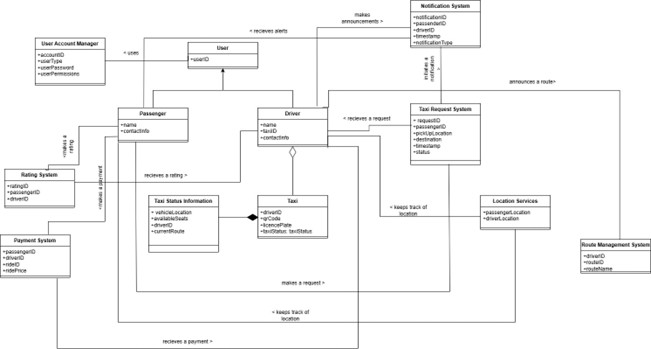
\includegraphics[width=1\textwidth]{Domain Model.jpg} 
\end{figure}

\section{Functional Requirements}

\subsection*{R1: User Account Management}
\begin{itemize}
    \item R1.1: Users should be able to register as either a driver or a passenger
    \item R1.2: Users should be able to update their Profile information
    \item R1.3: The system should support role-based access control for passenger and driver interfaces
    \item R1.4: Users should be able to reset or change their passwords
\end{itemize}

\subsection*{R2: Location Services}
\begin{itemize}
    \item R2.1: The system should track driver locations in real-time using GPS
    \item R2.2: The system should determine passenger locations for pickup requests
    \item R2.3: The system should calculate proximity between taxis and passengers
    \item R2.4: The system should send proximity alerts to notify passengers when their requested taxi is approaching
    \item R2.5: The system should display estimated time of arrival for approaching taxis 
\end{itemize}

\subsection*{R3: Taxi Request System}
\begin{itemize}
    \item R3.1: Passengers should be able to request taxi pickups based on their location
    \item R3.2: Passengers should be able to see nearby available taxis
    \item R3.3: Drivers should be notified of nearby passenger pickup requests
    \item R3.4: Drivers should be able to accept or decline pickup requests
    \item R3.5: Passengers should be able to specify their destinations
\end{itemize}

\subsection*{R4: Route Management}
\begin{itemize}
    \item R4.1: The system should allow drivers to announce their routes
    \item R4.2: The system should display taxi routes to passengers
    \item R4.3: The system should allow drivers to indicate their destinations
    \item R4.4: The system should support flexible drop-off points along routes
    \item R4.5: The system should optimize routes based on multiple passenger pickup/drop-off points
    \item R4.6: The system should display route information in a visual format suitable for quick comprehension
\end{itemize}

\subsection*{R5: Taxi Status Information}
\begin{itemize}
    \item R5.1: The system should display real-time taxi tracking showing vehicle location
    \item R5.2: The system should show available seats in approaching taxis
    \item R5.3: The system should allow drivers to update their seat availability status
    \item R5.4: The system should indicate taxi status (en route, picking up, full, etc.)
    \item R5.5: The system should notify waiting passengers when taxis reach capacity
\end{itemize}

\subsection*{R6: Notifications}
\begin{itemize}
    \item R6.1: The system should send push notifications for taxi proximity alerts
    \item R6.2: The system should notify passengers when their requested taxi accepts or declines the pickup
    \item R6.3: The system should notify drivers of new nearby passenger requests
    \item R6.4: The system should provide ETA updates to waiting passengers 
    \item R6.5: The system should send notifications even with limited connectivity 
    \item R6.6: The system should allow users to customize notification preferences
\end{itemize}

\subsection*{R7: Passenger Destination Management}
\begin{itemize}
    \item R7.1: The system should allow passengers to specify their drop-off locations
    \item R7.2: The system should support grouping passengers by similar destinations
    \item R7.4: The system should suggest optimal drop-off order to drivers
\end{itemize}

\subsection*{R8: User Interface}
\begin{itemize}
    \item R8.1: The system should provide separate interfaces for passengers and drivers
    \item R8.2: The system should offer a clean, easy-to-use interface with visual elements
    \item R8.3: The system should support multiple South African languages 
\end{itemize}

\subsection*{R9: Rating and Feedback}
\begin{itemize}
    \item R9.1: Passengers should be able to rate drivers/taxis
    \item R9.2: The system should collect feedback on routes and service
    \item R9.3: Users should be able to anonymously report safety incidents
\end{itemize}

\subsection*{R10: Fare Management}
\begin{itemize}
    \item R10.1: The system should calculate fare estimates based on route and distance
    \item R10.2: The system should support both digital and cash payment options
    \item R10.3: The system should provide payment confirmation receipts
    \item R10.4: The system should track payment status for trips
\end{itemize}

\subsection*{R11: Taxi Identification}
\begin{itemize}
    \item R11.1: The system should provide unique identifiers for each taxi
    \item R11.2: The system should support QR code-based taxi identification and verification
    \item R11.3: The system should display taxi information (registration, operator) to passengers
    \item R11.4: The system should verify taxi authenticity through the system
\end{itemize}

\subsection*{R12: Safety Features}
\begin{itemize}
    \item R12.1: The system should provide an anonymous crime reporting tool
    \item R12.2: The system should include emergency contact features
\end{itemize}

\section{Use Case Diagrams}
  \subsection*{Overall System}
    \begin{figure}[H]
      \centering
      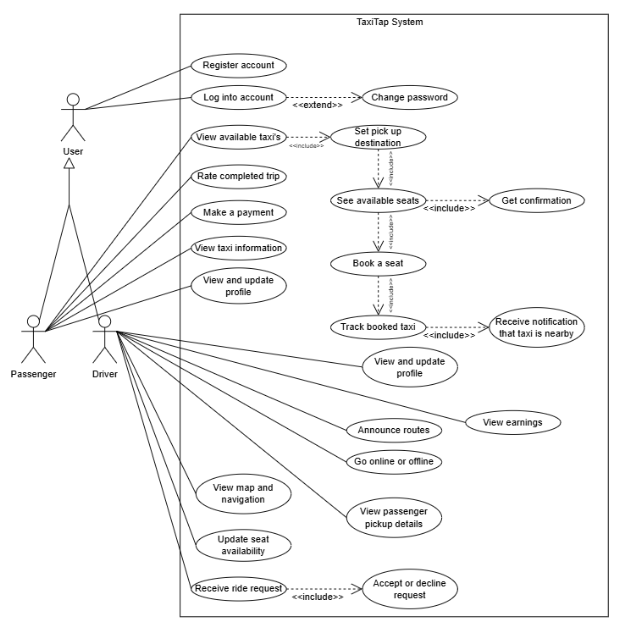
\includegraphics[width=1\textwidth]{OverallSystem.png} 
    \end{figure}
  \subsection*{Feedback}
    \begin{figure}[H]
      \centering
      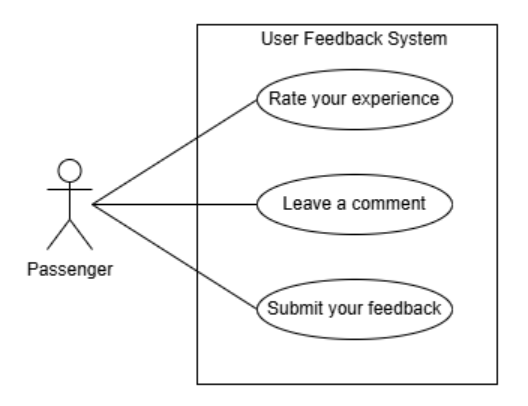
\includegraphics[width=1\textwidth]{UserFeedback.png} 
    \end{figure}
  \subsection*{Login}
    \begin{figure}[H]
      \centering
      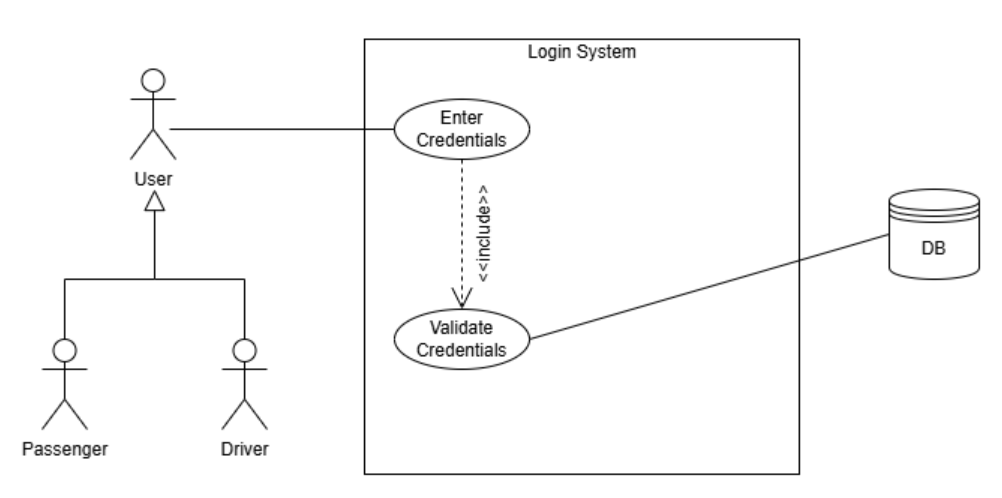
\includegraphics[width=1\textwidth]{Login.png} 
    \end{figure}
  \subsection*{Signup}
    \begin{figure}[H]
      \centering
      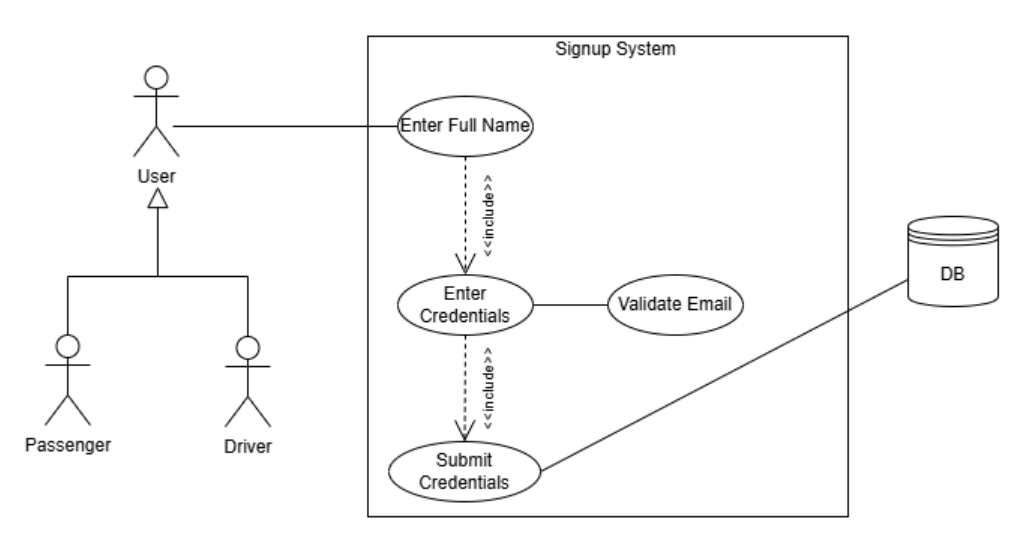
\includegraphics[width=1\textwidth]{SignUp.png} 
    \end{figure}
  \subsection*{Ride Request}
    \begin{figure}[H]
      \centering
      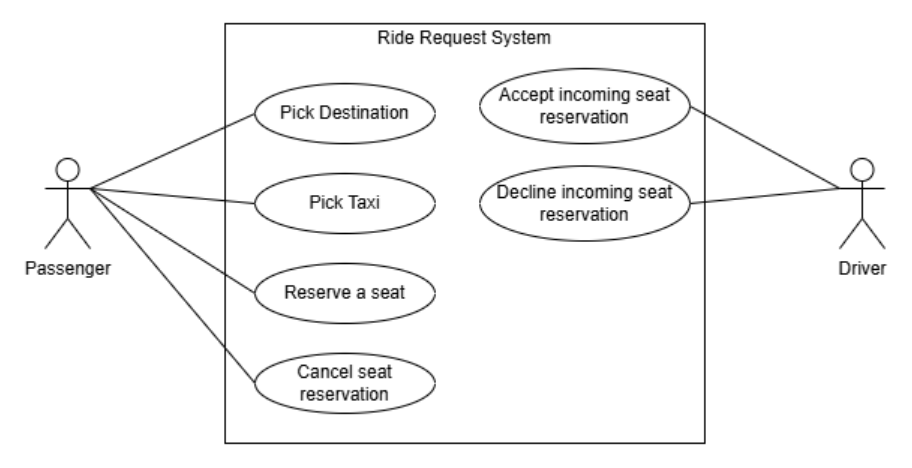
\includegraphics[width=1\textwidth]{RideRequest.png} 
    \end{figure}

\section{Technology Requirements}

\subsection{Frontend}
\textbf{Expo (React Native with TypeScript)}\\
\textbf{Why we chose to use Expo?}
\begin{itemize}
    \item \textbf{Cross-platform Compatibility:} Code once, deploy to both Android and iOS.
    \item \textbf{Native Features:} Access to GPS, accelerometer, push notifications, offline storage, camera, QR scanning, etc.
    \item \textbf{Web Support:} Leverages Expo Web for rendering web-based dashboards and admin panels.
    \item \textbf{Live Reloading \& Fast Iteration:} Expo Go provides hot reloading and rapid prototyping with a unified development experience.
    \item \textbf{Battery \& Data Optimization:} React Native ecosystem provides fine-grained control over performance, reducing overhead.
\end{itemize}

\subsection{Backend}
\textbf{Convex (TypeScript)}\\
\textbf{Why we chose to use Convex?}
\begin{itemize}
    \item \textbf{Truly Serverless:} No provisioning, no scaling headaches. Functions, database, and auth all run in one integrated environment.
    \item \textbf{Built-in Database:} Convex provides a powerful document-oriented database that supports relations, IDs, indexes, and real-time reactivity.
    \item \textbf{Type Safety:} Schema definition is in TypeScript, ensuring end-to-end type safety from backend to frontend.
    \item \textbf{Zero DevOps:} No need to manage infrastructure or containers. Deploy directly from your project.
    \item \textbf{Realtime Sync:} Built-in support for reactive queries allows passengers to see live taxi updates, seat availability, and ETA.
\end{itemize}

\subsubsection*{Convex Database Architecture}
\begin{itemize}
    \item \textbf{Document Store:} Convex uses collections of JSON-like documents, like MongoDB, but with built-in schema validation.
    \item \textbf{Indexes:} Automatic indexing on IDs and custom indexing for optimized query performance.
    \item \textbf{Relationships:} You can use Convex \texttt{v.id()} to reference documents between tables, ensuring referential integrity.
    \item \textbf{Realtime Subscriptions:} Query results update automatically when the underlying data changes.
\end{itemize}

\subsubsection*{Convex Free Tier (as of 2025)}
\begin{itemize}
    \item Compute: Up to 1 million function calls/month.
    \item Storage: 1 GB document data storage.
    \item Bandwidth: 5 GB of egress.
    \item Authentication: Integrated with third-party auth providers (Firebase Auth, Clerk, etc.).
    \item Deployment: 1 Production Deployment and 1 Dev Deployment per project.
\end{itemize}

\noindent Perfect for COS 301: Within budget, no surprise bills, and production-grade scalability.

\subsection{Key Functional Modules \& Implementation Plan}

\subsubsection*{User Management Subsystem}
\begin{itemize}
    \item Authentication: Convex Auth with Clerk or Firebase integration.
    \item Registration/Login: Role-based registration (passenger or driver) with schema enforcement.
    \item Profile Updates: Mutation to update user document with profile fields.
    \item Security: JWT-based session validation, encryption at rest and in transit.
\end{itemize}

\subsubsection*{Location Services Subsystem}
\begin{itemize}
    \item Driver Location: Periodic GPS updates using Expo Location API.
    \item Passenger Location: One-time or continuous tracking during trip.
    \item Proximity Alerts: Triggered from Convex using background function.
    \item ETA Calculation: Naive approach using Haversine distance + average speed (no Google Maps API due to cost).
\end{itemize}

\subsubsection*{Taxi Request Subsystem}
\begin{itemize}
    \item Request Workflow:
    \begin{itemize}
        \item Passenger sends request with coordinates and optional destination.
        \item Nearby drivers notified (push notification via Expo).
        \item Driver accepts or rejects request.
        \item Status changes handled in real time.
    \end{itemize}
\end{itemize}

\subsubsection*{Route Management Subsystem}
\begin{itemize}
    \item Driver Route Declaration: Input form for common route + destination.
    \item Passenger View: Map view of taxis on route + destinations.
    \item Optimized Routing (Optional): Historical route optimization using stored patterns (stretch goal).
\end{itemize}

\subsubsection*{Notification System}
\begin{itemize}
    \item Technology: Expo Notifications API.
    \item Use Cases:
    \begin{itemize}
        \item Taxi is approaching.
        \item Ride accepted or declined.
        \item Route changes or delays.
    \end{itemize}
    \item Offline Support: Caching notifications locally using AsyncStorage.
\end{itemize}

\subsubsection*{Safety and Fare Management Subsystem}
\begin{itemize}
    \item QR Identification: QR codes linked to taxi documents in Convex.
    \item Reporting: Anonymous incident reports saved to a secure Convex table.
    \item Fare Estimate: Static fare matrix per route (e.g., km-based fare slabs).
    \item Payment: Optional - integrate with SnapScan/Yoco for digital payments.
\end{itemize}

\subsection{Testing Frameworks}
\begin{itemize}
    \item Backend: Jest (unit and integration tests for Convex functions).
    \item Frontend: React Native Testing Library.
    \item Manual Testing: Device tests using Expo Go and emulators.
\end{itemize}

\subsection{CI/CD}
\begin{itemize}
    \item Convex Deployment: Triggered via GitHub Action or manual \texttt{npx convex dev} / \texttt{convex deploy}.
    \item Expo Deployment: Use \texttt{eas build} + \texttt{eas submit} for App Store/Play Store releases.
    \item Linting \& Tests: Pre-commit lint checks with ESLint + Jest unit tests.
\end{itemize}

\subsection{Version Control}
\begin{itemize}
    \item GitHub repo with main and dev branches.
    \item Feature branches for each core module.
\end{itemize}

\section{Architectural Requirements}

\subsection{Quality Requirements}
Quality requirements determine the overall quality of Taxi Tap by specifying criteria that define how well the system performs and behaves.

\begin{enumerate}
    \item \textbf{Security}
    \begin{enumerate}[a.]
        \item Encryption: All data must be encrypted in transit and at rest using the best security practices.
        \item Compliance: Data capturing and storing must be adhered to the POPI act, ensuring data privacy and consent handling.
        \item Secure authentication: Users must authenticate securely, and sessions must be protected.
    \end{enumerate}

    \item \textbf{Usability}
    \begin{enumerate}[a.]
        \item Simplicity: the interface should be easy to use for people with varying levels of tech literacy.
        \item Accessibility: The use of clear labels, large tap targets and minimal steps to complete key tasks.
        \item Feedback and error handling: Provide real-time feedback for user actions, loading states and clear error messages when issues occur.
    \end{enumerate}

    \item \textbf{Scalability}
    \begin{enumerate}[a.]
        \item The backend must scale horizontally and vertically to handle fluctuations in user or data load without performance degradation. This is automatically done by our chosen backend.
    \end{enumerate}

    \item \textbf{Performance}
    \begin{enumerate}[a.]
        \item Low bandwidth optimization: The system must perform reliably under low-bandwidth or intermittent connectivity.
        \item Battery efficiency: The app must minimize CPU, GPS and network usage to extend battery life.
    \end{enumerate}

    \item \textbf{Reliability and Availability}
    \begin{enumerate}[a.]
        \item Offline Support: The app must function even without a constant internet connection, using local caching or data queuing mechanisms.
        \item High uptime: The system should be available with minimal downtime to support driver operations throughout the day.
        \item Data integrity: Ensure that data is not lost or duplicated during sync offline and online states.
    \end{enumerate}

    \item \textbf{Maintainability and Extensibility}
    \begin{enumerate}[a.]
        \item Clean architecture: Backend and frontend systems should be modular and loosely coupled to allow easier updates, fixes, or feature additions in the future.
        \item Logging and monitoring: Implement centralized logging and monitoring to quickly identify and resolve issues.
        \item Configurability: Support code configurations without needing code changes.
    \end{enumerate}

    \item \textbf{Affordability}
    \begin{enumerate}[a.]
        \item Low data consumption: The app must use data sparingly to remain cost-effective for users in regions with expensive or limited mobile data.
        \item Resource efficiency: The system should minimize server and client-side consumption to reduce infrastructure and battery costs.
    \end{enumerate}
\end{enumerate}

\subsection{Architectural Patterns}
Architectural patterns are compositions of architectural elements which allow a system to effectively meet its quality requirements.

The Taxi Tap system consists of three components:
\begin{itemize}
    \item The mobile interface for passengers and drivers
    \item The backend service that handles ride coordination
    \item The real-time notification system
\end{itemize}

To meet its performance, scalability, and usability goals under strict constraints (low bandwidth, battery efficiency, AWS Free Tier), our team plans to use a combination of architectural patterns that balance simplicity with flexibility.

\paragraph{How the patterns will be applied in the Taxi Tap system:}

\begin{enumerate}
    \item \textbf{Event-Driven Architecture (EDA) with Publisher-Subscriber}\\
    The system will use the Publisher-Subscriber pattern to implement an Event-Driven Architecture. When a passenger requests a ride, an event is published (\texttt{RideRequested}) that triggers subscribed modules like ride matching, GPS location updates, and notifications. This design enables loose coupling, scalability, and real-time responsiveness, which are essential for a transportation app operating under varying loads.\\
    \textbf{Key Events:} RideRequested, TaxiApproaching, PassengerWaiting, etc.

    \item \textbf{Client-Server Architecture}\\
    The system will use the Client-Server architecture, where the mobile application acts as a client and communicates with a backend server. The application handles user input, displays route and ride information, and temporarily stores data when offline. The backend processes requests like user authentication, route announcements, ride matching, and storing data.\\
    We will use Convex as our serverless backend. This will allow us to write backend logic without managing infrastructure. Convex automatically handles scaling and storage, which helps us focus on building features rather than maintaining servers. It also supports real-time updates and is well-suited for low-latency mobile apps like Taxi Tap. 
\end{enumerate}

\subsection{Implementation Strategies}
To complement these architectural patterns, the following strategies will be considered.

\begin{enumerate}
    \item \textbf{Offline-First Strategy:}\\
    Users may have limited internet connectivity, therefore, the mobile application should be designed with offline-first capabilities. Actions such as ride requests or location tracking are stored locally and queued for syncing when the connection is re-established. This ensures continuity in usage and improves the app’s reliability in low-bandwidth environments.

    \item \textbf{Security Strategy:}\\
    To meet the requirement for secure handling of user data in line with POPIA and best practices, the following strategies will be used:
    \begin{itemize}
        \item \textbf{Data in Transit:} All data exchanged between the mobile application and backend services will be encrypted using HTTPS with TLS (Transport Layer Security).
        \item \textbf{Access Control:} Role-based access policies and authentication mechanisms (e.g., JWTs) ensure only authorised users can access specific system resources.
    \end{itemize}
    These strategies work within the architectural patterns to address the specific constraints of the South African minibus taxi ecosystem.
\end{enumerate}

\subsection{Design Patterns}

\paragraph{Observer Pattern}
\begin{itemize}
    \item Pattern Type: Behavioural
    \item Participants:
    \begin{itemize}
        \item Subject: Notification System
        \item Observer: User
        \item Concrete Observer: Passenger, Driver 
    \end{itemize}
    \item Explanation: The Observer pattern allows an object (User) to be notified automatically of state changes in another object (Notification System). This is ideal for handling events like route updates or ride status.
    \item Example:
    \begin{itemize}
        \item User receives alerts from the Notification System.
        \item Notification System initiates a notification when a route is announced.
    \end{itemize}
\end{itemize}

\paragraph{Mediator Pattern}
\begin{itemize}
    \item Pattern Type: Behavioural
    \item Participants:
    \begin{itemize}
        \item Mediator: Taxi Request System
        \item Colleague: Passenger, Driver
    \end{itemize}
    \item Explanation: The Mediator pattern centralizes complex communication between objects. Instead of Passenger directly interacting with Driver, requests are handled through the Taxi Request System.
    \item Example:
    \begin{itemize}
        \item Taxi Request System acts as an intermediary between Passenger and Driver.
        \item Passenger makes a request for pickup to a driver, but the Taxi request system acts as the middleman for this request.
    \end{itemize}
\end{itemize}

\subsection{Constraints}
The client laid out the following constraints, by which Taxi Tap must abide, in their specification.

\begin{enumerate}
    \item \textbf{All data must be encrypted at transit and at rest}\\
    All data exchanged between the mobile application and backend services will be encrypted using HTTPS with TLS (Transport Layer Security). Role-based access policies and authentication mechanisms (e.g., JWTs) ensure only authorised users can access specific system resources.

    \item \textbf{POPI act}\\
    To ensure we abide by this, we will not collect any user data that is not necessary for the functionality of the app. With that, we will have permission set up to ensure that users are comfortable with collecting info, such as the user’s location. Furthermore, we will consider providing a Terms and Conditions for the app that lays out how user data will be used.

    \item \textbf{The app must function with low bandwidth, low data usage and be battery-efficient}\\
    We will accomplish this by having a UI that does not use too many resources and lightweight calls to the API.

    \item \textbf{Budget}\\
    We must use AWS Free Tier platforms or any platforms that are open source or within free tier allowance.
\end{enumerate}

\end{document}